\documentclass[aspectratio=169,11pt]{beamer}

\usetheme{metropolis}
\metroset{block=fill, numbering=fraction, progressbar=frametitle}

\usepackage[T1]{fontenc}
\usepackage{amsmath,amssymb,bm}
\usepackage{booktabs}
\usepackage{graphicx}
\usepackage{xcolor}

% figures live in the simulation-output folder
\graphicspath{{../cascaded_chi3/figures/samples/}}

% shorthands
\newcommand{\chitwo}{\chi^{(2)}}
\newcommand{\chithree}{\chi^{(3)}}
\newcommand{\chicasc}{\chi^{(3)}_{\mathrm{casc}}}
\newcommand{\Dom}{\Delta\omega}
\newcommand{\gtwo}{\gamma_2}
\definecolor{good}{HTML}{2ca02c}
\definecolor{bad}{HTML}{d62728}
\newcommand{\yes}{\textcolor{good}{\textbf{yes}}}
\newcommand{\no}{\textcolor{bad}{\textbf{--}}}

\title{Cascaded $\chitwo{:}\chitwo \to \chithree_{\mathrm{eff}}$ in a
       Single-Resonance Metasurface}
\subtitle{Singly-resonant (SH-only) cascaded-$\chithree$ study}
\date{\today}

\begin{document}

\maketitle

% ---------------------------------------------------------------
\begin{frame}{The idea, and the question}
  \textbf{Cascaded Kerr.} Two $\chitwo$ steps in series synthesise an effective
  third-order response at the fundamental $\omega_1$:
  \[
    \omega_1+\omega_1 \xrightarrow{\ \chitwo\ } 2\omega_1
    \xrightarrow{\ \chitwo\ } \omega_1 ,
    \qquad
    \chithree_{\mathrm{eff}} \sim \chitwo \!\cdot\! G(2\omega_1) \!\cdot\! \chitwo .
  \]
  The second-harmonic field is eliminated adiabatically, leaving an
  intensity-dependent index on the pump.

  \begin{alertblock}{The trade we are testing}
    The effect is strongest when \emph{both} $\omega_1$ (fundamental, FM) and
    $2\omega_1$ (SH) are sharp resonances --- the \textbf{two-mode} metasurface.
    A \textbf{single} SH resonance is far easier to fabricate. \\[2pt]
    \textbf{What do we keep, and what do we lose, with one resonance instead of two?}
  \end{alertblock}
\end{frame}

% ---------------------------------------------------------------
\begin{frame}{Two-mode vs.\ one-mode: the critical differences}
  \scriptsize
  \begin{table}
  \begin{tabular}{@{}lll@{}}
    \toprule
     & \textbf{Two-mode} (FM\,+\,SH) & \textbf{One-mode} (SH only) \\
    \midrule
    Resonances            & qBIC @ $\omega_1$ \ +\ SH @ $2\omega_1$ & SH only; FM broadband \\
    Material $\chicasc$    & \multicolumn{2}{c}{\emph{same} form: $-\omega_1|\chitwo|^2\eta_{\mathrm{geom}}/[6n_2^2(\Dom+i\gtwo/2)]$} \\
    FM field build-up     & resonant, $\times Q_1$                  & none (single pass) \\
    Per-photon Kerr phase & $\propto Q_1^{2}\,Q_2$                   & $\propto Q_2$ only \\[2pt]
    Bistability, switching   & \yes                                 & \no\ \ (no FM cavity to detune) \\
    Optical limiter, AM mod. & \yes                                 & \no \\
    SPM / XPM / FWM / sat.\ abs. & strong                          & survive, $Q_1^{2}\!-\!Q_1^{4}$ suppressed \\
    Sign tunability ($\Dom$) & \yes\ (within $\pm\gamma_1$)         & \yes\ (broad) \\
    Fabrication           & two aligned resonances (hard)           & one resonance (easy) \\
    \bottomrule
  \end{tabular}
  \end{table}
  \normalsize
  \vspace{2pt}
  \textbf{One sentence:} the cascade \emph{mechanism and material $\chithree$ are
  intact}; what the single resonance throws away is the $Q_1^{2}$ leverage that the
  FM cavity gives to \emph{observables}.
\end{frame}

% ---------------------------------------------------------------
\begin{frame}{Same material $\chithree$, different leverage}
  The single-resonance effective susceptibility (SH eliminated adiabatically):
  \[
    \boxed{\ \chicasc(\Dom)\;=\;-\,\frac{\omega_1\,|\chitwo|^{2}\,
            \eta_{\mathrm{geom}}}{6\,n_2^{2}\,(\Dom+i\gtwo/2)}\ },
    \qquad
    \eta_{\mathrm{geom}}=\bigl(|\mathrm{overlap}|/A\bigr)^{2}.
  \]
  \begin{itemize}
    \item \textbf{Real part} $\propto -\Dom$: sign-tunable self-focusing\,/\,defocusing.
    \item \textbf{Imaginary part}: two-photon-like loss, set by $Q_2$.
    \item $\eta_{\mathrm{geom}}$ (the SHG mode overlap) enters \emph{linearly} --- the binding constraint.
    \item No FM resonance $\Rightarrow$ observables lose the $Q_1^{2}$ build-up (single-pass phase).
  \end{itemize}
\end{frame}

% ---------------------------------------------------------------
\begin{frame}{What we can observe --- and what we cannot}
  \small
  \begin{columns}[T]
    \begin{column}{0.5\textwidth}
      \textcolor{good}{\textbf{Observable ($\chithree$):}}
      \begin{itemize}
        \item \textbf{Sign flip} self-focus\,$\leftrightarrow$\,defocus across
              $\Dom=0$ (scale-robust)
        \item Material $\chithree$ gain $R\!\approx\!1.8$--$2.5$ (indirect)
        \item ps pulses: SPM ($\sim$mrad), sat.\ abs., FWM --- as diagnostics
        \item \emph{SHG}: a $\chitwo$ process, \alert{out of scope} --- only to \emph{calibrate}
      \end{itemize}
    \end{column}
    \begin{column}{0.5\textwidth}
      \textcolor{bad}{\textbf{Not observable (need FM cavity):}}
      \begin{itemize}
        \item CW Kerr-phase \emph{device} ($\mu$rad)
        \item Bistability, all-optical switching
        \item Optical limiter, AM modulator
        \item Even pulsed: phase $\ll0.1$\,rad
      \end{itemize}
    \end{column}
  \end{columns}
  \vspace{3pt}
  \footnotesize Need the FM cavity as the oscillator $\Rightarrow$ \emph{die}; use
  $\chicasc$ as a single-pass input $\Rightarrow$ \emph{survive but suppressed}.
\end{frame}

% ---------------------------------------------------------------
\begin{frame}{Designs under study}
  Four candidate single-resonance LiNbO$_3$ designs (full-wave simulations);
  pump $\lambda_1\!\approx\!1\,\mu$m, SH in the green, 400\,nm period.
  \begin{table}\footnotesize
  \begin{tabular}{@{}lcccccc@{}}
    \toprule
    S & $\lambda_1$ & $\lambda_2$ (SH) & $Q_2$ & $\Delta f=\gtwo/2\pi$ & $\eta_{\mathrm{geom}}$ & $R=|\chicasc|/\chithree_{\mathrm{nat}}$ \\
    \midrule
    1 & 997\,nm  & 498\,nm & 3442 & 175\,GHz & 0.014 & 0.49 \\
    2 & 975\,nm  & 488\,nm & 3486 & 176\,GHz & 0.011 & 0.39 \\
    3 & 1058\,nm & 529\,nm & 4641 & 122\,GHz & 0.037 & 1.76 \\
    \textbf{4} & \textbf{1064\,nm} & \textbf{532\,nm} & \textbf{5633} & \textbf{100\,GHz} & \textbf{0.044} & \textbf{2.49} \\
    \bottomrule
  \end{tabular}
  \end{table}
  \vspace{2pt}
  Operating point: conservative $\Dom=2\gtwo$. Material baseline
  $|\chitwo|=5\!\times\!10^{-11}$\,m/V, $\chithree_{\mathrm{nat}}=2\!\times\!10^{-21}$\,m$^2$/V$^2$.
  \alert{Only samples 3 and 4 beat the native Kerr.}
\end{frame}

% ---------------------------------------------------------------
\begin{frame}{Result: cascaded $\chithree$ spectra}
  \centering
  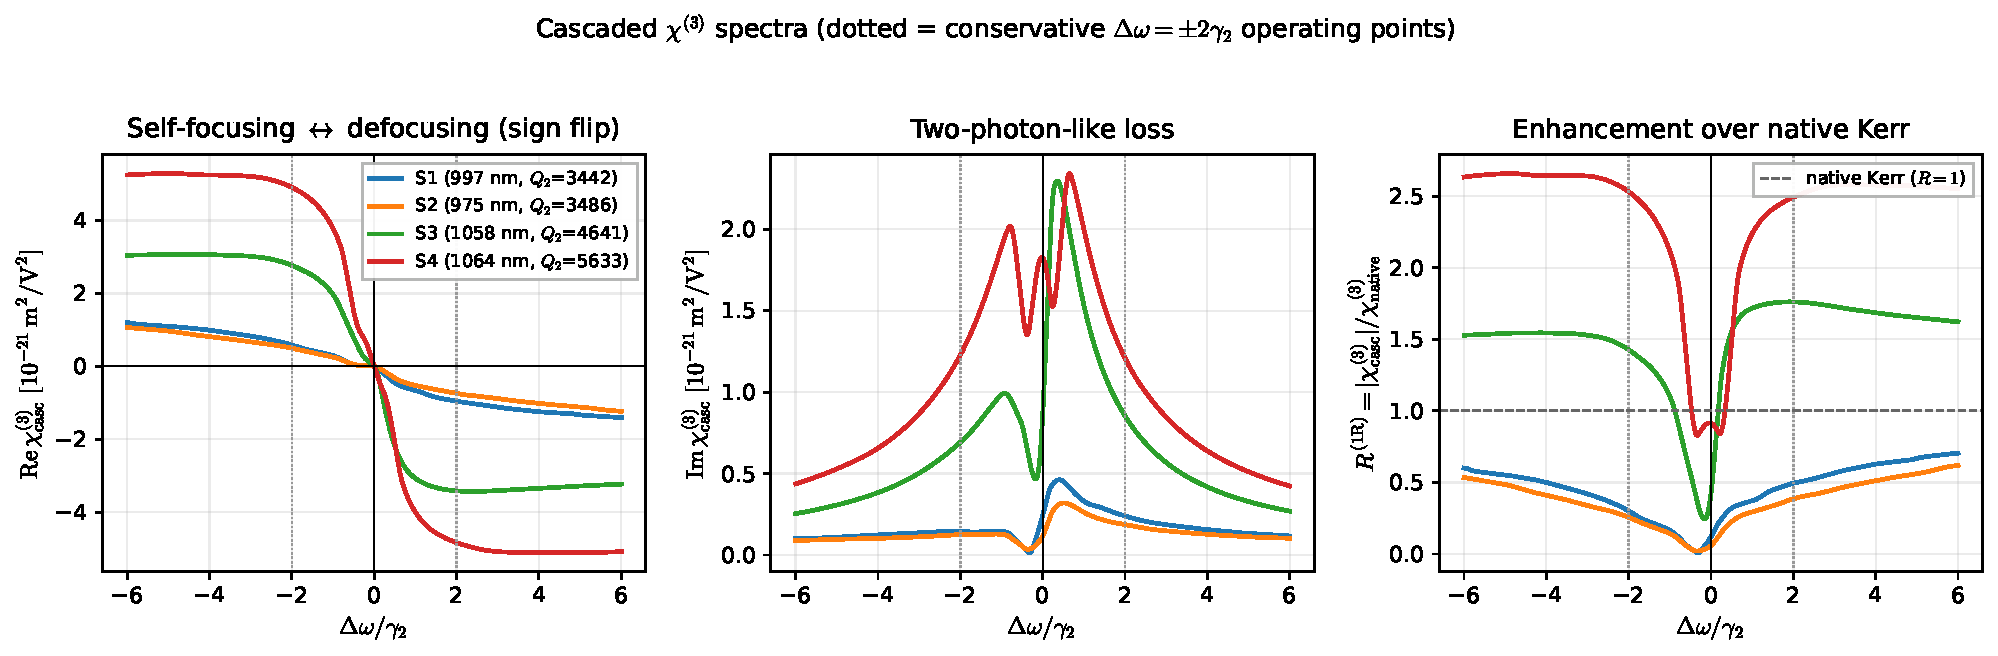
\includegraphics[width=\linewidth]{sample_chi3_spectra.pdf}
  \vspace{-2pt}
  \begin{itemize}\footnotesize
    \item (a) sign flip at $\Dom=0$; \ (b) loss peaks \emph{off} resonance (overlap
          collapses at the line centre); \ (c) only S3, S4 clear $R=1$.
  \end{itemize}
\end{frame}

% ---------------------------------------------------------------
\begin{frame}{Result: the overlap is the bottleneck}
  \centering
  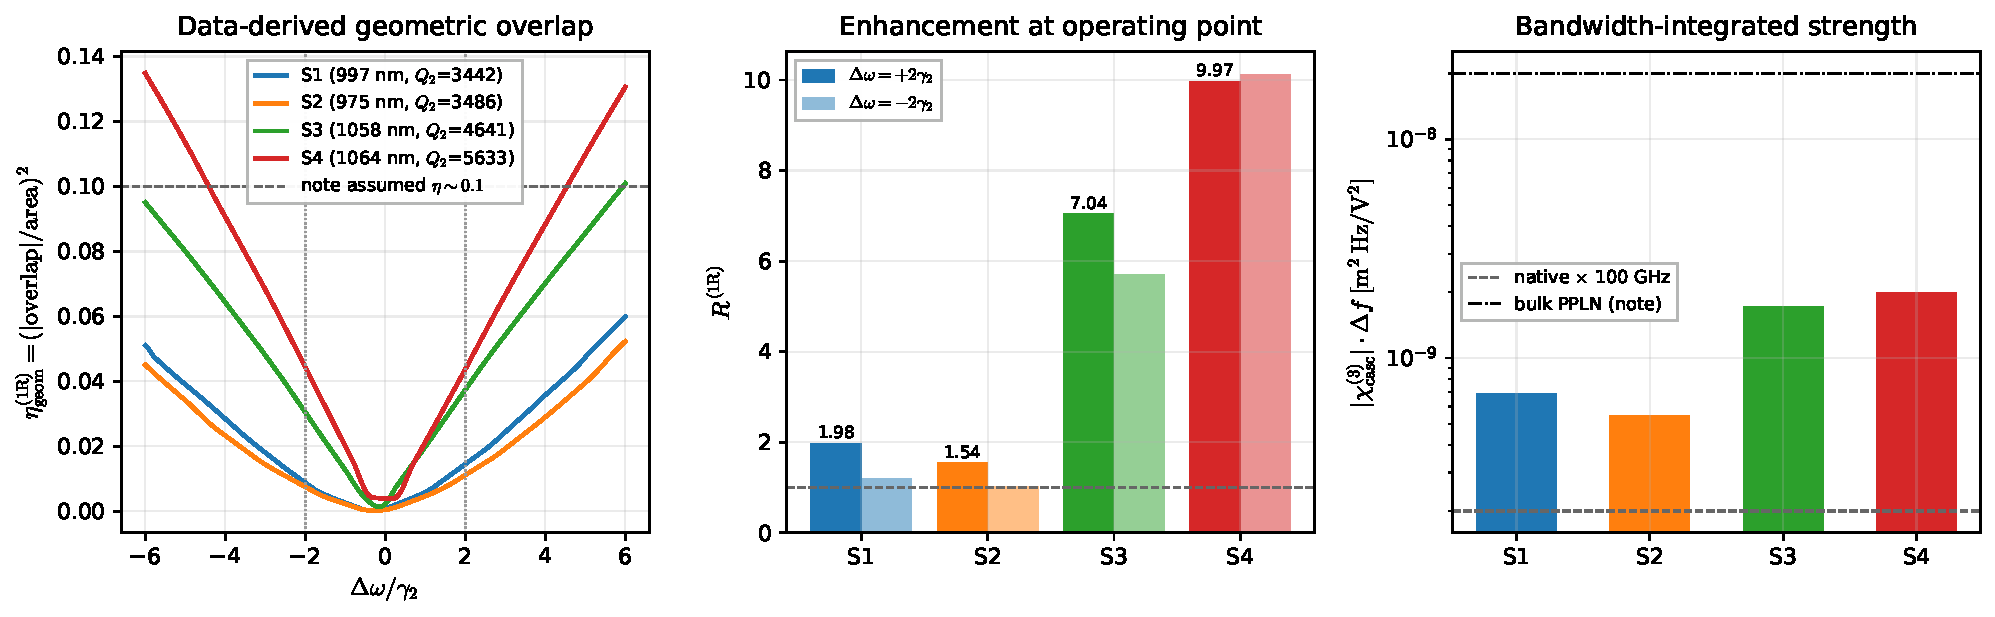
\includegraphics[width=\linewidth]{sample_eta_and_ranking.pdf}
  \vspace{-2pt}
  \begin{itemize}\footnotesize
    \item $\eta_{\mathrm{geom}}=0.011$--$0.044$ --- a factor $2$--$10$ below a
          ``good'' overlap ($\sim0.1$); $\chicasc\propto\eta_{\mathrm{geom}}$.
    \item Even the best design is $\sim\!40$--$100\times$ below bulk PPLN in
          $|\chicasc|\!\cdot\!\Delta f$: the edge is chip-scale form factor, not raw strength.
  \end{itemize}
\end{frame}

% ---------------------------------------------------------------
\begin{frame}{Result: detuning is not the lever}
  \centering
  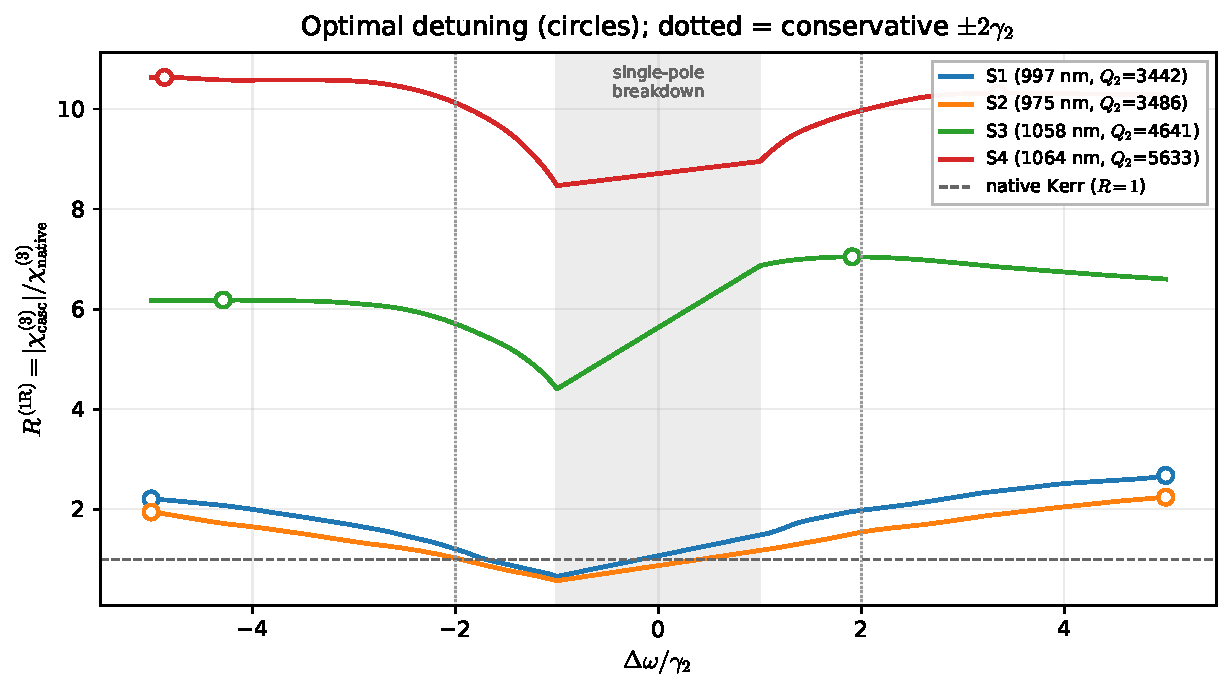
\includegraphics[width=0.64\linewidth]{sample_optimal_detuning.pdf}
  \begin{itemize}\footnotesize
    \item Broad, flat plateau in the wings; conservative $\Dom=2\gtwo$ is within
          $\sim\!5\%$ of optimal for S3, S4. $R$ \emph{dips} inside $|\Dom|<\gtwo$.
    \item \alert{Spend the effort on the overlap, not the detuning.}
  \end{itemize}
\end{frame}

% ---------------------------------------------------------------
\begin{frame}{Feasibility: the ps-pulse regime}
  \centering
  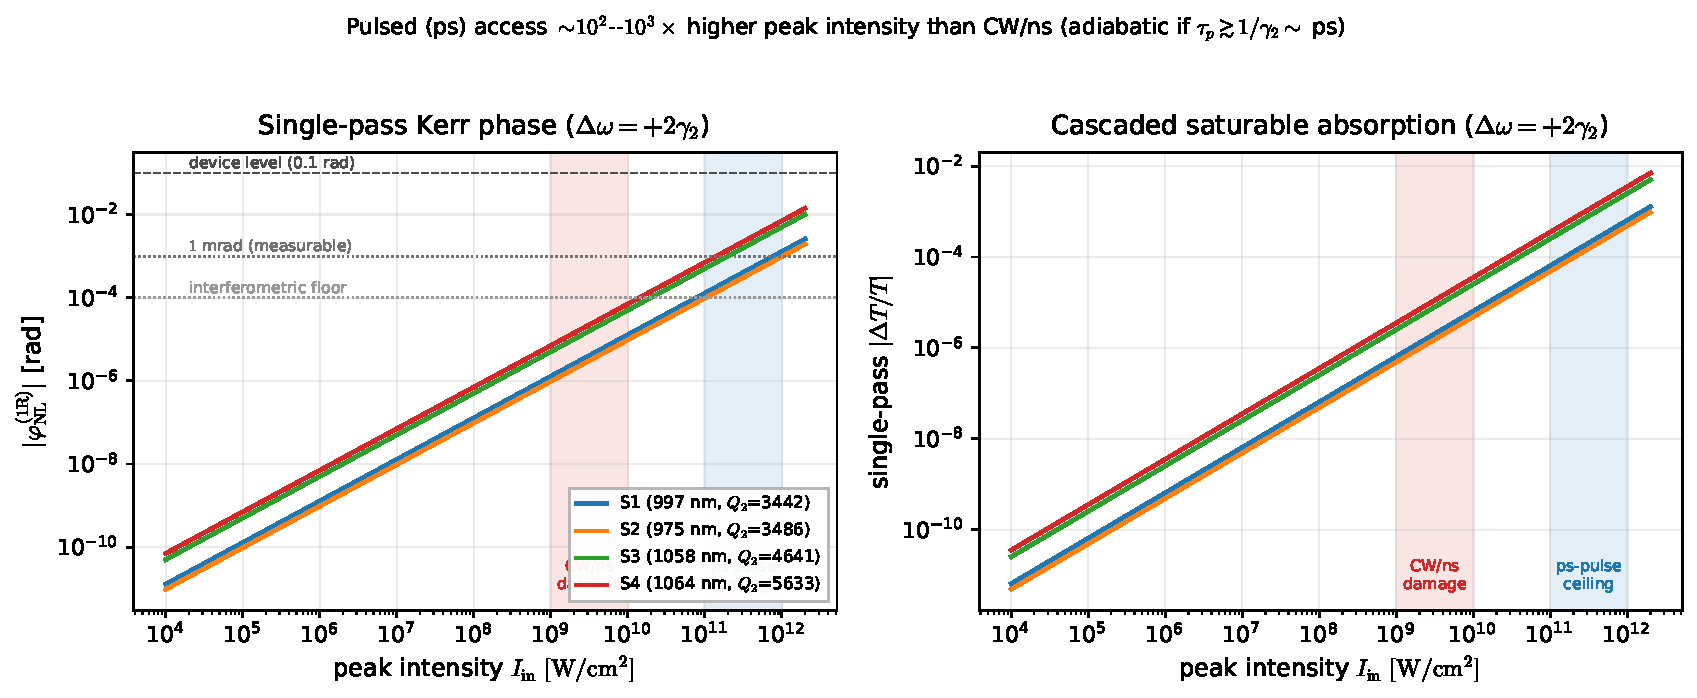
\includegraphics[width=0.72\linewidth]{sample_feasibility.pdf}
  \begin{itemize}\footnotesize
    \item \textbf{CW:} sub-nrad phase + green-SH photorefractive damage --- nothing observable.
    \item \textbf{ps pulses} ($\tau_p\!\sim\!1$--$3$\,ps): $10^2$--$10^3\times$ more peak
          intensity, no CW damage $\Rightarrow$ phase $\sim$mrad, $\Delta T/T\!\sim\!10^{-3}$
          --- \alert{measurable}, but still $\ll0.1$\,rad (no device).
    \item \alert{These curves are quasi-static (CW $\chithree$ at peak $I$).} Since
          $\tau_p\!\sim\!$ SH lifetime $1/\gtwo\!\sim\!1$--$1.6$\,ps, the SH may not fully
          build up --- a time-domain pulse simulation tests this (next slide).
  \end{itemize}
\end{frame}

% ---------------------------------------------------------------
\begin{frame}{Time-domain pulse simulation}
  Integrating $\dot a_2=(i\Dom-\gtwo/2)\,a_2+i\,\beta(t)$ with $\beta(t)\!\propto\!I(t)$
  (FM instantaneous) --- the actual ps response, not the CW formula:
  \begin{columns}[c]
    \begin{column}{0.5\textwidth}
      \centering
      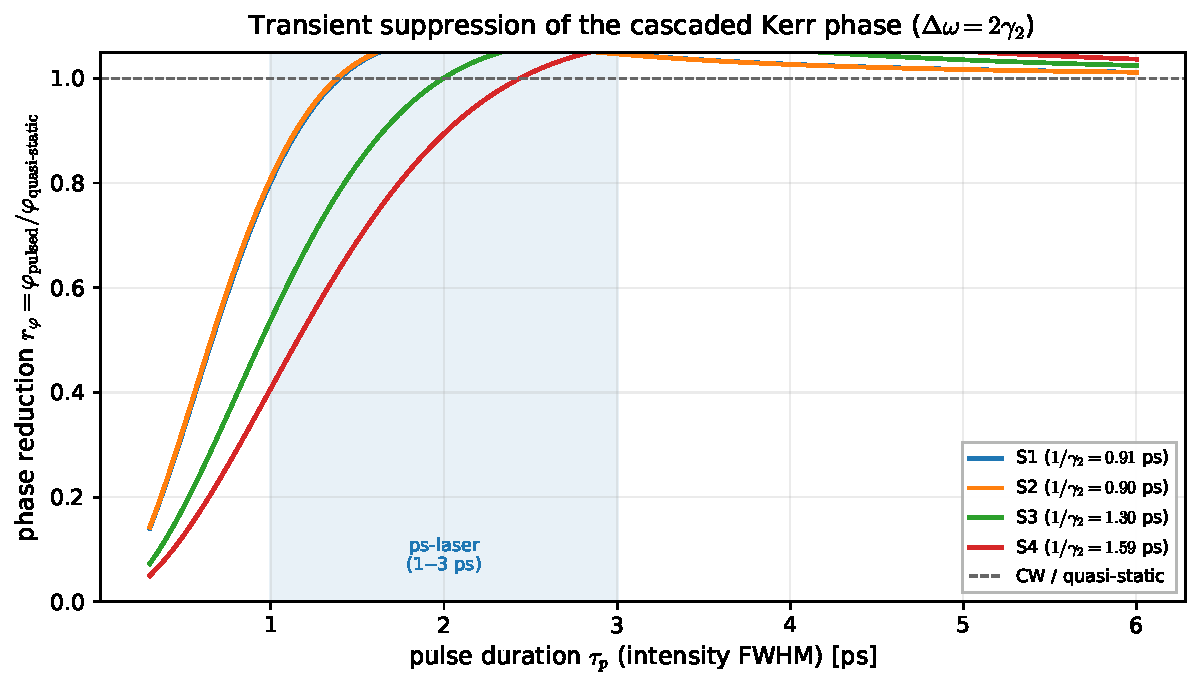
\includegraphics[width=\linewidth]{sample_pulsed_reduction.pdf}
    \end{column}
    \begin{column}{0.5\textwidth}
      \centering
      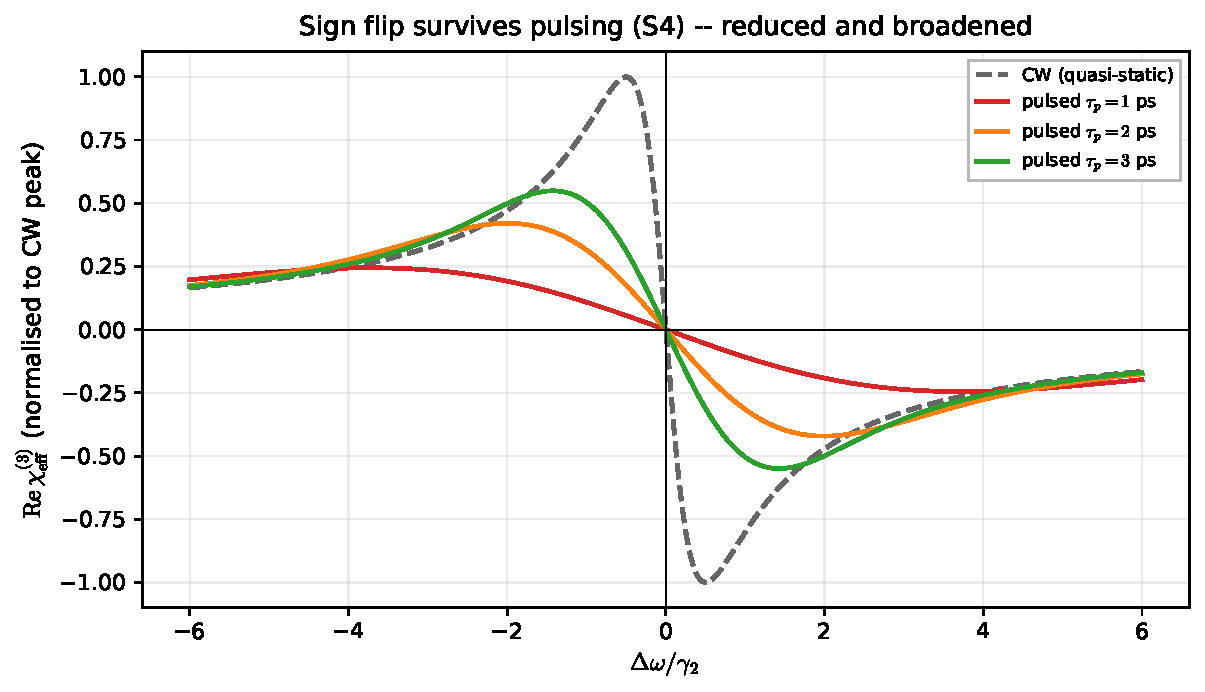
\includegraphics[width=\linewidth]{sample_pulsed_signflip.pdf}
    \end{column}
  \end{columns}
  \vspace{1pt}
  {\footnotesize
   \textbf{At $\tau_p\!\gtrsim\!2$\,ps the cascade is essentially undiminished}
   ($r_\varphi\!\approx\!0.9$--$1.05$, slight overshoot); quasi-static $\sim$mrad holds.
   Penalty only at \textbf{1\,ps}: $\sim\!1.25\times$ (low-$Q$ S1/S2) to $\sim\!2.5\times$
   (high-$Q$ S4) $\Rightarrow$ \alert{use $\tau_p\!\gtrsim\!2$\,ps}. The \textbf{sign flip
   survives} (right), reduced and broadened.}
\end{frame}

% ---------------------------------------------------------------
\begin{frame}{What to measure --- and how}
  \begin{columns}[T]
    \begin{column}{0.54\textwidth}
      \centering
      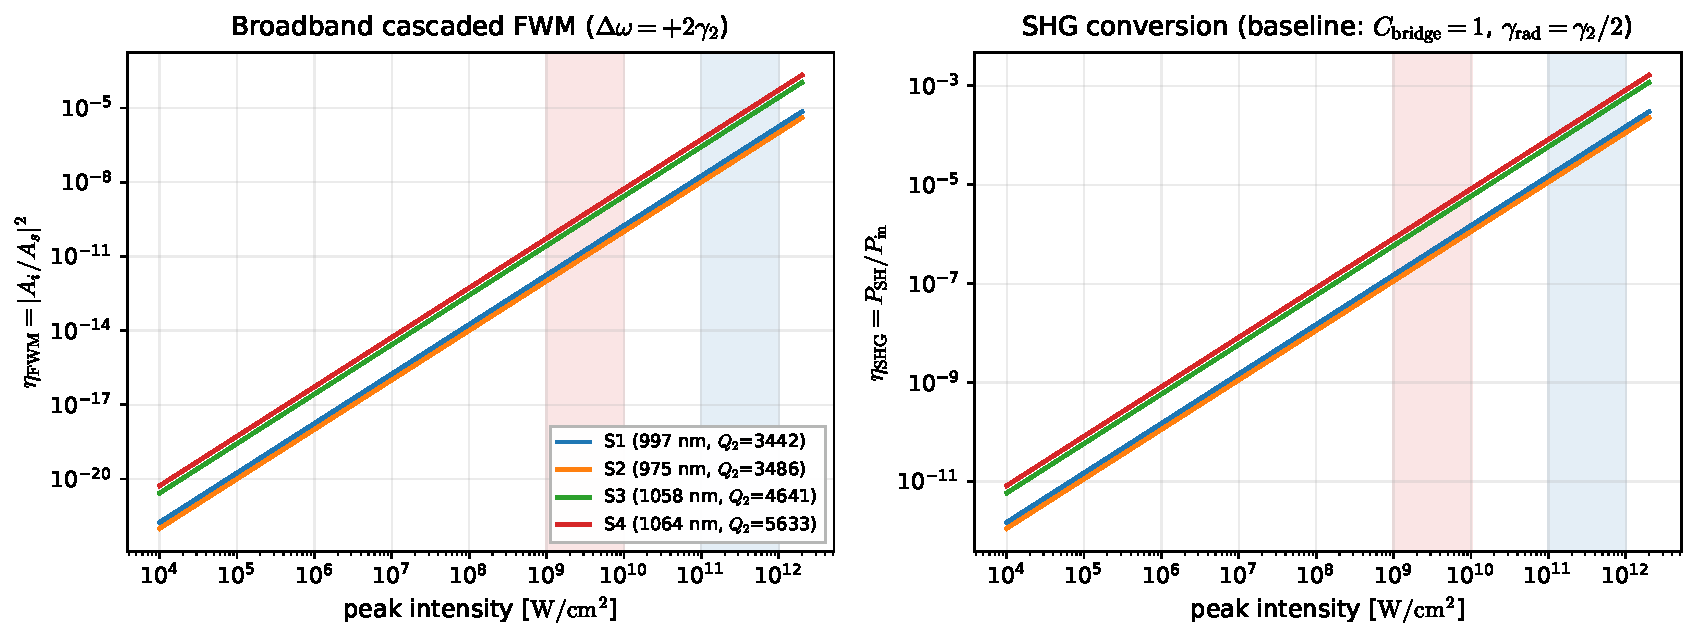
\includegraphics[width=\linewidth]{sample_fwm_shg.pdf}
    \end{column}
    \begin{column}{0.46\textwidth}\small
      \textbf{1. The $\chithree$ signature (in scope).}\\
      Detuning-resolved Z-scan / spectral SPM with ps pulses: self-focusing
      $\leftrightarrow$ defocusing across $\Dom=0$ (scale-robust). Broadband,
      phase-matching-free FWM as a second $\chithree$ probe.\\[4pt]
      \textbf{2. SHG efficiency --- calibration only.}\\
      A $\chitwo$ process, \alert{not our target} --- but it shares the same overlap
      and SH resonance, so $\eta_{\mathrm{SHG}}$ vs.\ detuning/power \emph{pins the
      absolute $\chicasc$ scale} and validates the cascade's first ($\chitwo$) step.
    \end{column}
  \end{columns}
\end{frame}

% ---------------------------------------------------------------
\begin{frame}{How to measure the $\chithree$ sign flip}
  \begin{columns}[T]
    \begin{column}{0.5\textwidth}\small
      \textbf{Closed-aperture Z-scan vs.\ detuning}
      \begin{itemize}
        \item \textbf{Pump at $\omega_1$} (always). Scan the pump wavelength so its
              \emph{generated} harmonic $2\omega_1$ crosses the SH resonance
              ($\Dom=2\omega_1-\omega_2:-\!\to\!+$).
        \item Closed-aperture trace: \emph{valley$\to$peak} $=$ self-focusing
              ($n_2\!>\!0$), \emph{peak$\to$valley} $=$ defocusing --- reads the
              \textbf{sign} of $n_2$ directly.
        \item The cascade is \textbf{odd in $\Dom$}: its sign flips as $\Dom$ crosses $0$.
      \end{itemize}
    \end{column}
    \begin{column}{0.5\textwidth}\small
      \textbf{Watch the native-Kerr background}
      \begin{itemize}
        \item Native LiNbO$_3$ $n_2>0$ is constant --- it does \emph{not} flip.
        \item Total $n_2=n_2^{\rm nat}+n_2^{\rm casc}(\Dom)$: a \emph{full} reversal of
              the total needs $R>1$ (samples 3, 4).
        \item Robust readout either way: isolate the cascade as the
              \textbf{antisymmetric-in-$\Dom$} part (native is even/constant).
      \end{itemize}
    \end{column}
  \end{columns}
  \vspace{3pt}
  \footnotesize Equivalent probes: spectral SPM/XPM blue-vs-red asymmetry, or spectral
  interferometry for the signed nonlinear phase. ps pulses + lock-in for the small ($\sim$mrad) signal.
\end{frame}

% ---------------------------------------------------------------
\begin{frame}{Conclusions}
  \begin{itemize}
    \item The single-resonance metasurface \textbf{keeps the cascade mechanism and a
          modest material enhancement} ($R\!\le\!2.5$, samples 3--4) but
          \textbf{loses the $Q_1^{2}$ leverage} the FM resonance provides.
    \item \textbf{No CW Kerr device} (bistability, switching, limiter, modulator)
          --- these need the FM cavity and die qualitatively.
    \item The overlap, not the detuning or $Q_2$, is the binding constraint, and it
          is currently $2$--$10\times$ too small.
    \item \textbf{Best role of the one-mode platform:} a $\chithree$ \emph{diagnostic}
          (sign flip + FWM; SHG only to \emph{calibrate} the scale) and a
          \emph{materials-level} $\chithree$ --- not a standalone device.
    \item \textbf{Pulsed (ps) pumping} lifts the $\chithree$ to $\sim$mrad (measurable),
          not device level. A time-domain TCMT pulse simulation confirms this holds for
          \alert{$\tau_p\!\gtrsim\!2$\,ps}; only a $\sim\!2.5\times$ penalty at 1\,ps (high-$Q$).
  \end{itemize}
\end{frame}

% ---------------------------------------------------------------
\begin{frame}{Recommendations, and what we still need}
  \textbf{Design rules (priority order):}
  \begin{enumerate}\footnotesize
    \item \textbf{Maximise the overlap} to $|\mathrm{overlap}|\gtrsim0.3$ (qBIC asymmetry,
          sub-domain poling, pump near-field shaping) --- the dominant linear lever.
    \item Fix the operating point at $\Dom\!\approx\!2\gtwo$.
    \item Push $Q_2$ (mind bandwidth + disorder $\sigma_\omega/\omega\!\lesssim\!1/Q_2$);
          thicker, MgO-doped LiNbO$_3$ (green-SH photorefractive).
    \item \textbf{Pump with ps pulses}, not CW (more peak intensity, no photorefractive);
          \textbf{keep $\tau_p\!\gtrsim\!2$\,ps} ($\gtrsim2\times$ SH lifetime, time-domain sim).
    \item \textbf{For a CW Kerr \emph{device}: add the FM resonance back} (go two-mode).
  \end{enumerate}
  \textbf{Still to compute / measure:}
  \begin{itemize}\footnotesize
    \item one full \textbf{nonlinear SHG simulation} to calibrate the absolute scale;
    \item \textbf{loaded vs.\ intrinsic} $Q$; refined $\chitwo,\chithree_{\mathrm{nat}}$ at $\sim\!1\,\mu$m.
  \end{itemize}
\end{frame}

% ---------------------------------------------------------------
\begin{frame}[standout]
  Summary: the cascade \emph{mechanism} survives with one resonance;\\
  the \emph{device leverage} does not.\\[6pt]
  \normalsize Maximise the overlap; use it as a diagnostic;\\
  go two-mode for a device.
\end{frame}

\end{document}
